% =====================================================================
% CAMERA-READY LINKS --- SWAP IN AFTER ACCEPTANCE (kept here, NOT in the
% review PDF body). All artifact URLs in the body are de-anonymized for this single-blind submission.
%   Code repository:        https://github.com/rikhinkavuru/gb_kmer_benchmark
%                           (repo name to confirm before camera-ready)
%   Cleaned splits (Zenodo): doi:10.5281/zenodo.20448617
%   Frozen-FM embedding cache (HyenaDNA + DNABERT-2) + manifest: Zenodo DOI TBD on release
%   Diagnostic CLI (diagnose.py): in the code repository above
% PSB is not double-blind (author names appear on the title page); body artifact
% URLs are de-anonymized for this single-blind submission. Real author identity
% appears on the title page + cover letter.
% =====================================================================
\documentclass{ws-procs11x85}
\usepackage{ws-procs-thm}
\usepackage{graphicx}
\usepackage{float}
\usepackage{url}
% Force US Letter page size (class/pdftex defaulted to A4 595x842pt); set before layout.
\pdfpagewidth=8.5in \pdfpageheight=11in
% --- float-packing (layout only; no content or font change; body stays 12pt/15pt) ---
\raggedbottom
\setlength{\textfloatsep}{8pt plus 2pt minus 2pt}
\setlength{\floatsep}{8pt plus 2pt minus 2pt}
\setlength{\intextsep}{8pt plus 2pt minus 2pt}
% FIX 4: keep the \copyrightinfo footnote (CC BY-NC license line) from splitting across pages
\interfootnotelinepenalty=10000

\begin{document}

% =====================================================================
% COVER LETTER --- page 1 of the submission (NOT counted in the 12 body pages).
% =====================================================================
\thispagestyle{empty}
% Blind policy: PSB 2027 is single-blind (confirmed by organizers) --- the named title page / author identity is correct as submitted; no anonymization required.
\noindent\textbf{\large Cover Letter}\\[6pt]
\noindent To the organizers of the Pacific Symposium on Biocomputing (PSB) 2027,\\[6pt]

\noindent I submit the enclosed manuscript, ``Three Routes to Failure: An Interpretable
Diagnosis of Task Difficulty and Negative-Set Contamination in Genomic
Sequence-Classification Benchmarks,'' for consideration.\\[6pt]

\noindent\textbf{Corresponding author email:} \texttt{rikhinkavuru@gmail.com}\\[3pt]
% PSB 2027 session chosen: "Biological Molecular Function: Beyond Homology"
% (chairs McDermott, Bromberg, Carter, Wheeler; confirm fit by emailing jason.mcdermott@pnnl.gov).
\noindent\textbf{Requested session:} ``Biological Molecular Function: Beyond Homology''\\[3pt]
\noindent This work fits the session's \emph{beyond-homology} theme from the evaluation side: with interpretable, intervention-confirmed diagnostics, it shows that leading genomic foundation-model benchmarks are partly solved by homology leakage and compositional shortcuts rather than genuine molecular function---so moving beyond homology also requires benchmarks that do not reward those confounds.\\[3pt]
\noindent\textbf{Originality:} This paper contains original, unpublished results and is not currently under
consideration for publication elsewhere.\\[3pt]
\noindent\textbf{Authorship:} I am the sole author of this paper.\\[3pt]
\noindent\textbf{Disclosure of LLM use (required):} A large language model (LLM) was used as an
AI assistant, under the author's direction, to help implement the experiments, run the analyses,
and draft and revise the text. All quantitative results reported in the paper were produced by the
released, deterministic, open-source code (fixed seed; results written to versioned CSV/JSON files)
and were inspected and verified by the author. The author takes full responsibility for the
correctness and content of the paper.\\[6pt]

% PREPRINT ACK (paste verbatim on the preprint when posted, per PSB author kit): Preprint of an article submitted for consideration in Pacific Symposium on Biocomputing © 2027 World Scientific Publishing Company http://psb.stanford.edu/
\noindent I intend to post a preprint of this manuscript to bioRxiv or arXiv.\\[6pt]

\noindent Thank you for your consideration.\\[6pt]
\noindent\textit{Rikhin Kavuru}

\clearpage

% =====================================================================
% TITLE PAGE --- author names/addresses (NOT counted in the 12 body pages).
% PSB is not double-blind; identity appears here and in the cover letter (body text carries no author identity).
% =====================================================================
\title{Three Routes to Failure: An Interpretable Diagnosis of Task Difficulty and
Negative-Set Contamination in Genomic Sequence-Classification Benchmarks}

\author{Rikhin Kavuru\footnote{Corresponding author: \texttt{rikhinkavuru@gmail.com}.}}

\address{Independent Researcher,\\ Fort Wayne, Indiana, USA}

\begin{abstract}
Benchmarks that judge genomic foundation models (FMs) by their accuracy at classifying DNA
sequences are increasingly relied upon, yet what makes a task ``easy'' or ``hard'' has been
largely unexamined. We use an explicitly-interpreted, GPU-free ($k$-mer spectrum features and
gradient-boosted trees) pipeline to diagnose performance across two benchmark suites (Genomic
Benchmarks; the Nucleotide Transformer downstream tasks) and isolate three mechanistically-distinct
routes to benchmark failure, each confirmed by intervention. First, motif \emph{presence} does not
predict success---across the nine Genomic Benchmarks tasks the number of enriched
transcription-factor motifs is uncorrelated with learnability (Spearman $-0.03$)---whereas motif
\emph{discriminability} does: a semi-synthetic dose-response that dials the motif-only AUROC ($d$)
of motifs implanted only in positives drives the benchmark MCC monotonically (Spearman $+0.924$,
$n{=}135$; OLS slope $+1.99$, carried by three independent per-motif fits of $+1.96$ to $+2.02$).
The real-task correlation corroborates this ($\rho{=}+0.74$, $n{=}11$, strengthening to $+0.87$ on
the homology-clean subset), and out-of-sample a leave-one-task-out fit gives a stable mean absolute
error of $0.14$ MCC (with $R^2{=}+0.44$ but a wide CI $[-0.27,+0.70]$ that includes $0$ at $n{=}11$).
Second, positional information governs learnability: position-binned $k$-mers give a \emph{selective}
rescue---one large recovery for the fixed-position task (splice sites, MCC $0.244\to0.868$), one
marginal gain for the TATA-promoter, and $\sim$0 for the other twelve. Third, and most consequential,
negative-set contamination: the negatives of two separately-curated human enhancer benchmarks carry
an excess of TATA/AT-rich sequence ($+20.9$ to $+22.7\%$). A GRCh38/GENCODE coordinate analysis
refutes a core-promoter reading (flagged negatives are TSS-\emph{depleted}); the excess is AT-rich
background composition. We measure the artifact's magnitude directly---composition-equalizing the
negatives collapses the \texttt{human\_enhancers\_cohn} $k$-mer MCC $0.461\to0.064$ and the TATA/GC
motif-only AUROC to chance, and dinucleotide-shuffled negatives make it vanish. As an existence proof
that pretrained models---not only our classifier---ride this shortcut, two architecturally-unrelated
frozen genomic FMs (HyenaDNA; DNABERT-2) lose near-identical, significant enhancer AUROC when the
composition artifact is removed, each against its own flat control. We frame the contamination as a
\emph{benchmark-design} artifact---the enhancer-vs-AT-rich-background composition gap is a real
biological property exploited by a trivial axis, not dataset corruption---and release cleaned splits,
the frozen-FM embedding cache (so the entire FM result reproduces with zero PyTorch), and a diagnostic
command-line tool.
\end{abstract}

\keywords{interpretable machine learning; genomic benchmarks; regulatory sequence classification;
negative-set contamination; $k$-mer features; DNA foundation models.}

% required, do-not-remove
% Copyright: standard WS open-access CC BY-NC 4.0 line, (c) 2027, sole-author 'The Author' --- consistent with the PSB/WS author kit (open access, PMC deposit); optionally cross-check the exact boilerplate against the LaTeX template zip.
\copyrightinfo{\copyright\ 2027 The Author. Open Access chapter published by World Scientific
Publishing Company and distributed under the terms of the Creative Commons Attribution
Non-Commercial (CC BY-NC) 4.0 License.}

% =====================================================================
% BODY (the 12-page count starts here). De-anonymized for this single-blind submission.
% =====================================================================
\section{Introduction}\label{introduction}

Benchmark leaderboards now drive much of the development of DNA foundation models
(FMs)\cite{nt,dnabert,dnabert2,hyenadna,caduceus} --- a model's standing is its aggregate accuracy
across suites such as Genomic Benchmarks\cite{gb} and the Nucleotide Transformer downstream
tasks\cite{nt} --- yet the benchmarks themselves are treated largely as black boxes. We rarely ask
\emph{what property of a task makes it easy or hard}, or whether a high score reflects biological signal
rather than an artifact of dataset construction. Without that, a leaderboard number is hard to interpret:
two models with the same score may exploit very different things, and a ``solved'' task may be solved for
the wrong reason.

We treat a simple, CPU-only classifier as an \textbf{interpretable diagnostic lens}, not a competitor to
foundation models: frequency-normalized $k$-mer spectra classified with gradient-boosted trees
(LightGBM\cite{lightgbm}), so that --- because $k$-mers map to short motifs --- every prediction traces
back to interpretable units. CPU-only is a property of the method, not a claimed contribution; we use
frozen forward passes of pretrained FMs only as a probe (Section~\ref{fm-probe}), neither fine-tuning them
nor claiming to beat them.

Our contribution is a \textbf{mechanistic taxonomy of task difficulty} with three routes to failure,
each demonstrated directly, replicated on an independent suite where possible, and confirmed by
intervention:

\begin{romanlist}[(iii)]
\item \textbf{Shared-motif} --- the discriminative motifs are present in \emph{both} classes, so they
cannot separate them;
\item \textbf{Positional} --- the signal is a fixed-position motif that a position-blind spectrum
discards;
\item \textbf{Contamination} --- the \emph{negative} class is drawn from a different compositional
distribution (an AT-rich background) that produces spurious separability, replicated across two human
enhancer benchmarks.
\end{romanlist}

We establish each route causally rather than by correlation or single example: (i)~Route~1 by a
dose-response at arbitrary sample size ($n{=}135$) plus a held-out test; (ii)~Route~2 by a selective
rescue across all 15 tasks and a bin-resolution sweep; (iii)~Route~3's \emph{magnitude} by
composition-equalized cleaning and dinucleotide-shuffled negatives, and its \emph{specificity} by an
information-content-matched control-motif panel. As an existence proof that pretrained models ride the
shortcut, two frozen genomic FMs lose significant enhancer AUROC when the artifact is removed, each
against its own flat control.

A result ran \emph{contrary to our initial expectation}: motif \emph{presence} does not predict success
--- the hardest tasks are often the most motif-rich --- whereas \emph{discriminability} does. Throughout,
``contamination'' means a negative set carrying a label-correlated artifact: here an AT-rich compositional
bias, not biological core-promoter leakage (which our Route~3 coordinate analysis tests directly). We
release cleaned splits, the frozen-FM embedding cache, and a diagnostic tool so future evaluations can
avoid the artifact.

\section{Related Work}\label{related-work}

\textbf{DNA foundation models and benchmark suites.} Genomic FMs --- DNABERT\cite{dnabert},
DNABERT-2\cite{dnabert2}, the Nucleotide Transformer\cite{nt}, HyenaDNA\cite{hyenadna},
Caduceus\cite{caduceus} --- are pre-trained on large genomic corpora and ranked on downstream
classification suites: Genomic Benchmarks\cite{gb} (nine datasets: promoters, enhancers, regulatory and
open-chromatin regions, demonstration tasks) and the Nucleotide Transformer downstream tasks\cite{nt}
(promoter, enhancer, splice-site, with published FM numbers). We do not propose or fine-tune an FM; we
analyse these \emph{benchmarks} and use frozen forward passes of two FMs (HyenaDNA, DNABERT-2) only as an
interpretive probe (Section~\ref{fm-probe}).

\textbf{Negative-set composition bias in regulatory-sequence classification.} That the \emph{negative}
set can dominate a regulatory-sequence classifier is a recurring, under-emphasized theme. The
$k$-mer-SVM enhancer predictor of Lee, Karchin and Beer\cite{lee2011} and the gapped-$k$-mer SVM of
Ghandi \emph{et al.}\cite{ghandi2014} select features and negative controls to avoid trivial composition
cues; their tooling generates GC-, length-, and repeat-matched negatives for exactly this
reason\cite{ghandi2016}. Most directly, DeePromoter\cite{deepromoter} foregrounds our Route~3: because
TATA-like motifs are commoner genome-wide than in true promoters, models trained against easy
genomic-background negatives exploit them, so the authors build harder, composition-matched negatives.
Kr\"utzfeldt, Schubach and Kircher\cite{krutzfeldt2020} study the same axis quantitatively, comparing
GC-matched genomic negatives against $k$-mer-preserving shuffles --- the two interventions we use --- and
find the negative-set choice strongly determines what a regulatory model learns. Our contribution is
orthogonal: rather than choosing negatives to train a better predictor, we give a \emph{coordinate-resolved,
intervention-confirmed diagnosis} of negative-set composition contamination \emph{on released benchmark
splits} across two suites, with a cross-architecture frozen-FM probe and released cleaned splits. Inflation
by negative-set construction has also been noted for enhancer--promoter interaction
prediction\cite{caofullwood}.

\textbf{Non-foundation baselines.} ConvNova\cite{convnova} shows that from-scratch convolutional networks,
without large-scale pretraining, are competitive with --- and sometimes exceed --- genomic FMs; a separate
line uses embedding-plus-classifier baselines\cite{embed,feng2025} to question how much pretraining adds.
These establish \emph{that} non-foundation methods are competitive; our contribution is different --- we
use a simple, interpretable model not to win but to \emph{explain why} tasks are easy or hard (the
three-route mechanism). We add no from-scratch CNN comparison: our cross-architecture evidence comes from
frozen-FM probes and a model-family route-invariance analysis (Section~\ref{robustness}).

\section{Methods}\label{methods}

The diagnostic pipeline is CPU-only (no GPU, no PyTorch/TensorFlow; see the FM-probe note below), uses a
single fixed random seed (42) everywhere, and reports 95\% percentile-bootstrap confidence intervals (CIs)
with the individual test sequence as the resampling unit. Exact reproducibility parameters --- software
versions, LightGBM/LR hyperparameters, PSSM pseudocount and background, histogram-bin counts, bootstrap
and permutation resample counts, and the pinned dataset revision --- are listed in the supplement
in the code repository (\url{https://github.com/rikhinkavuru/gb_kmer_benchmark}); everything needed to judge each procedure is below.

\textbf{Featurization.} Each sequence is its $k$-mer spectrum for $k\in\{3,4,5,6\}$: counts over the
fixed, data-independent vocabulary of all $4^k$ ACGT $k$-mers, L1-normalized to relative frequencies. The
fixed vocabulary makes the feature space identical across datasets and splits (no vocabulary leakage);
$k$-mers with non-ACGT characters are ignored. Matrices are sparse (CSR).

\textbf{Models.} The main model is gradient-boosted trees (LightGBM\cite{lightgbm}) with hyperparameters
fixed across all datasets; a scikit-learn\cite{sklearn} logistic-regression (LR) \emph{floor} (with L2-normalized rows, since linear
models are scale-sensitive) is also reported. Metrics are accuracy, the Matthews correlation coefficient
(MCC)\cite{mcc} and the area under the ROC curve (AUROC, one-vs-rest macro for multiclass); we emphasise
MCC. Per dataset we select $k$ for LightGBM on a held-out validation split --- a stratified 80/20 carve of
the training set --- choose the $k$ with the highest \emph{validation} MCC, retrain on the full training
split, and evaluate once on the test split, which is never used for model selection.

\textbf{Per-TF motif enrichment.} We score $k$-mers against the JASPAR 2024 CORE collection\cite{jaspar,pyjaspar}
as log-odds position-specific scoring matrices (PSSMs) and test, per TF, whether its motif score is
\emph{enriched} among high-gain $k$-mers via a gain-weighted statistic against an analytic permutation
null, with Benjamini--Hochberg FDR\cite{bh} at $q<0.05$. We avoid a ``best match over the whole
collection'' threshold (with $\sim$880 profiles it \emph{saturates}: 61--100\% of $k$-mers are the optimal
substring of \emph{some} low-information window); the per-TF test does not saturate and names the
responsible TF.

\textbf{Motif-only discriminability.} To ask whether motifs \emph{separate the classes}, we scan each
sequence (both strands) with a curated set of TF PSSMs, count hits above a fixed bits-per-position
threshold, and compute the AUROC of motif-hit-count for the positive-vs-negative contrast (``motif-only
AUROC''). The threshold is fixed across both classes, so any difference is signal, not a threshold
artifact. For the GC-box (Sp1/KLF) we use 1.0 bits/pos; for TATA a specificity-controlled 1.3 bits/pos
(TBP is a low-information AT-rich motif, so at 1.0 bits/pos hit counts track AT-content; a sweep shows the
suspect-vs-control contrast persists at 1.3 while controls flatten, and the conclusion is intact across a
0.8--1.5 bits/pos sweep, Section~\ref{route-3}). The same vertebrate TBP profile is used for all species
including the \texttt{drosophila} control, since TBP and the TATA consensus are highly conserved.

\textbf{Semi-synthetic discriminability dose-response (Route~1).} To make the
discriminability--learnability relationship causal at arbitrary $n$, we generate random ACGT backgrounds
matched in length and base composition to a real task and implant PWM-sampled instances of a chosen
JASPAR TF into positives (and not negatives) at a tunable rate, sweeping the rate to vary the realized
motif-only AUROC $d$. Because the motif is implanted \emph{only in positives}, this manipulates
discriminability and is silent on motif \emph{presence} (answered separately on real tasks,
Section~\ref{route-1}). For each setting we featurize, fit LightGBM, and measure test MCC; we repeat over
five seeds and three motifs of differing information content (SP1, MYC, TBP). $d$ is \emph{measured}, not
assumed, by the same scan used on real data.

\textbf{Positional featurization.} To test the positional route we add (alongside, not replacing) a
position-binned spectrum: each sequence is split into $B$ equal-fraction bins, the L1-normalized $k$-mer
spectrum is taken within each, and the bins are concatenated to the global spectrum. $B{=}1$ is the
baseline; a sweep $B\in\{1,2,4,8,16\}$ measures how the rescue scales with bin resolution.

\textbf{Contamination cleaning.} We use three complementary cleanings of the \emph{negative} set;
positives are left identical. (i)~\emph{TATA-flag}: flag negatives carrying a high-confidence TATA box
(TBP $\ge$ 1.3 bits/pos) and remove a seeded random subset equal to the excess (the neg-minus-pos
TATA-box-rate gap $\times\,n_{\mathrm{neg}}$, e.g.\ 22.2\% of \texttt{cohn}'s negatives); since removal
shrinks the negative set the cleaned AUROC moves toward but not fully to 0.5. (ii)~\emph{GC-matched}:
subsample negatives to the positive-class GC histogram. (iii)~\emph{Fully composition-equalized}: we fit
one logistic-regression propensity model $p=P(\text{positive}\mid\text{composition})$ on a 20-dimensional
composition signature (4 mononucleotide + 16 dinucleotide L1-normalized frequencies), pooled over the
train and test sequences, then resample negatives \emph{within each split separately} so their propensity
histogram matches the positives' --- balancing GC and all 16 dinucleotides jointly
(Rosenbaum--Rubin\cite{rosenbaum}), with balance verified by the per-feature standardized mean difference.
Because equalized cleaning changes the test set the resulting MCC is \emph{unpaired}; the
motif/composition AUROC collapse is the causal readout.

\textbf{Dinucleotide-shuffled controlled negatives (Route~3).} For the \texttt{cohn} and
\texttt{nt\_enhancers} positives we construct matched negatives by an Altschul--Erikson
dinucleotide-preserving shuffle\cite{altschul} of the positives (Eulerian-path method; dinucleotide ---
hence mononucleotide and GC --- composition is preserved exactly, verified per sequence). By construction
these negatives have no composition gap, so any residual class signal is higher-order (motif) structure.

\textbf{Negative-control-motif panel (Route~3 specificity).} To test that the TATA skew is specific to the
motif rather than manufactured by the scanning procedure, we build information-content-matched control
PWMs: 20 column-permutations of the TBP PSSM (preserving per-column and total information content exactly
while destroying the ordered TATA pattern), and 10 random PWMs matched to TBP's total information content.
We scan the contaminated sets with each control using the \emph{identical} both-strand, fixed-threshold,
motif-only-AUROC procedure and compare to real TATA.

\textbf{Coordinate analysis (Route~3).} We recover GRCh38 coordinates for the negatives --- by exact
substring for \texttt{cohn} and by minimap2 alignment\cite{minimap2} for \texttt{nt\_enhancers} --- and
intersect TATA-flagged versus non-flagged negatives with GENCODE v44 transcription start sites (TSS,
$\pm$500\,bp), reporting overlap rates, a Fisher exact test, and the TATA-to-nearest-TSS offset
distribution.

\textbf{Frozen FM-probe (existence proof).}\label{fm-probe-method} We extract frozen embeddings from two
pretrained genomic FMs --- HyenaDNA-tiny (16k context, single-nucleotide tokenizer) and DNABERT-2-117M
(512-token context, byte-pair-encoding tokenizer) --- with CPU forward passes only (no fine-tuning, no
GPU), mean-pooling the last hidden state over real tokens and additionally storing the sequence-summary
token ([SEP] for HyenaDNA, [CLS] for DNABERT-2). On the frozen embeddings we train both an LR and a
LightGBM head and evaluate with the \emph{paired} protocol of Section~\ref{fm-probe}. All torch usage is
isolated to a separate embedding-extraction process (the diagnostic pipeline imports zero torch), and the
embeddings are released as a cache so the entire downstream FM result reproduces with no torch and no
model load. Significance for the motif-only AUROCs uses an empirical label-shuffle permutation null; the
NT tasks are read at a pinned dataset revision (supplement).

\section{Results}\label{results}

\begin{table}[htbp]
\tbl{Benchmark landscape across both suites: best-$k$ LightGBM per task, ordered by MCC (descending).
$n_\text{train}$/$n_\text{test}$ are the split sizes; CIs (95\% bootstrap, test sequence the resampling
unit) are on the test split. AUROC is one-vs-rest macro for the multiclass tasks (regulatory,
enhancers-types, splice). The `solved'/`composition' labels mark non-failing tasks; the three failure
routes are shared-motif, positional, and contamination. \texttt{human\_enhancers\_ensembl} is labelled
contamination~(weak): its excess is only $+10.8\%$, suggestive rather than robust. Every value is read
directly from the result CSVs.}
{\scriptsize\begin{tabular}{@{}llrrclcl@{}}
\toprule
Suite & Task (dataset id) & $n_\text{train}$ & $n_\text{test}$ & $k$ & MCC [95\% CI] & AUROC & Route\\
\colrule
GB & \texttt{demo\_human\_or\_worm} & 75{,}000 & 25{,}000 & 5 & 0.914 [0.909, 0.919] & 0.992 & composition\\
GB & \texttt{human\_ensembl\_regulatory} & 231{,}348 & 57{,}713 & 5 & 0.907 [0.904, 0.910] & 0.991 & solved\\
NT & \texttt{nt\_promoter\_all} & 53{,}276 & 5{,}920 & 4 & 0.888 [0.877, 0.899] & 0.985 & solved\\
NT & \texttt{nt\_promoter\_no\_tata} & 47{,}767 & 5{,}299 & 4 & 0.887 [0.873, 0.899] & 0.985 & solved\\
GB & \texttt{human\_nontata\_promoters} & 27{,}097 & 9{,}034 & 6 & 0.874 [0.864, 0.883] & 0.989 & solved\\
NT & \texttt{nt\_promoter\_tata} & 5{,}509 & 621 & 4 & 0.846 [0.803, 0.886] & 0.984 & solved\\
GB & \texttt{demo\_coding\_vs\_intergenomic} & 75{,}000 & 25{,}000 & 5 & 0.800 [0.793, 0.808] & 0.965 & composition\\
GB & \texttt{human\_enhancers\_ensembl} & 123{,}872 & 30{,}970 & 6 & 0.593 [0.585, 0.602] & 0.875 & contam.~(weak)\\
GB & \texttt{dummy\_mouse\_enhancers\_ensembl} & 968 & 242 & 6 & 0.529 [0.422, 0.632] & 0.858 & composition\\
NT & \texttt{nt\_enhancers} & 14{,}968 & 400 & 4 & 0.514 [0.432, 0.595] & 0.850 & contamination\\
NT & \texttt{nt\_enhancers\_types} & 14{,}968 & 400 & 6 & 0.476 [0.415, 0.532] & 0.837 & shared-motif\\
GB & \texttt{human\_enhancers\_cohn} & 20{,}843 & 6{,}948 & 5 & 0.461 [0.440, 0.482] & 0.805 & contamination\\
GB & \texttt{human\_ocr\_ensembl} & 139{,}804 & 34{,}952 & 6 & 0.421 [0.412, 0.430] & 0.785 & shared-motif\\
GB & \texttt{drosophila\_enhancers\_stark} & 5{,}184 & 1{,}730 & 4 & 0.398 [0.352, 0.441] & 0.763 & shared-motif\\
NT & \texttt{nt\_splice\_sites\_all} & 27{,}000 & 3{,}000 & 5 & 0.244 [0.219, 0.271] & 0.704 & positional\\
\botrule
\end{tabular}}
\label{tab:land}
\end{table}

\subsection{Benchmark landscape}\label{benchmark-landscape}

Table~\ref{tab:land} reports the best-$k$ LightGBM per task with 95\% bootstrap CIs; the
discriminability--learnability relationship it summarises is established causally in
Figure~\ref{fig:dose} (Route~1). Achievable MCC spans 0.244 to 0.914, and ``solved'' tasks are separated
from ``failed'' ones by non-overlapping CIs. The same difficulty gradient appears in both suites:
regulatory and promoter tasks are well-solved (\texttt{human\_ensembl\_regulatory},
\texttt{human\_nontata\_promoters}, the three NT promoters), whereas the enhancer and open-chromatin tasks
are hard (\texttt{human\_enhancers\_cohn}, \texttt{human\_ocr\_ensembl}, \texttt{nt\_enhancers}) and
splice-site classification is poorly solved (\texttt{nt\_splice\_sites\_all}) --- all MCCs in
Table~\ref{tab:land}. The taxonomy comprises three \emph{failure} routes --- shared-motif, positional, and
contamination; the `solved' and `composition' labels mark non-failing tasks, not failure routes. These benchmark MCCs are seed-invariant
(Section~\ref{robustness}).

The absolute MCC of \texttt{human\_nontata\_promoters} is partly homology-inflated ($\sim$41\% of its test
sequences have a $\ge$0.7-Jaccard near-duplicate in training), inflating the Table~\ref{tab:land} number
only, not the within-split GC-box discriminability finding below. The broader audit (the contamination
flagship \texttt{cohn} is redundancy-clean; \texttt{nt\_enhancers} has verbatim overlap) is detailed in the
Limitations.

\subsection{Route 1 --- discriminability, not presence: a causal dose-response}\label{route-1}

We hypothesized that well-solved tasks have discriminative $k$-mers matching known TF motifs.
\textbf{Disconfirmed} --- and the disconfirmation \emph{is} the ``presence does not predict success'' half
of Route~1: the number of FDR-enriched TF motifs does not track learnability (Spearman of MCC against
\#enriched TFs across the nine GB tasks $\rho{=}-0.03$, n.s.). The \emph{failed} enhancer/OCR tasks are in
fact the \emph{most} motif-rich (\texttt{human\_enhancers\_ensembl} 265, \texttt{human\_ocr\_ensembl} 243
FDR-enriched TFs), while the solved promoter relies on far fewer families. (The dose-response below
implants motifs only in positives, so it speaks only to discriminability, not presence; the presence
claim rests solely on this real-task dissociation.)

What does predict learnability is motif \textbf{discriminability} --- whether a motif is skewed to one
class. In \texttt{human\_nontata\_promoters}, GC-box / Sp1--KLF motifs are concentrated in the positive
(promoter) class: SP2 hit-count separates the classes with motif-only AUROC 0.751, and per-TF enrichment
ranks SP1 first (gain-weighted $z=7.60$, BH-FDR $1.4\times10^{-11}$), followed by SP2, SP4, KLF7, KLF12.
In contrast, on the failed \texttt{human\_ocr\_ensembl} the E-box / AP-1 motifs that dominate its $k$-mer
importance are present in \emph{both} classes (TFAP4 E-box positive mean 0.103 vs negative mean 0.046,
motif-only AUROC 0.527; BATF3 AP-1 0.648 vs 0.423, AUROC 0.573) --- abundant but non-discriminative (the
shared-motif route). The NT promoters replicate the GC-box-in-positives pattern
(\texttt{nt\_promoter\_no\_tata} SP1 hit-count positive mean 1.134 vs negative 0.428, AUROC 0.639).

\textbf{The causal dose-response (Figure~\ref{fig:dose}).} The original evidence for ``discriminability
predicts learnability'' was a pooled real-task correlation over $n{=}11$ tasks, underpowered within
either suite. We now establish the relationship \emph{causally} and at arbitrary sample size with a
semi-synthetic dose-response (Methods): implanting a TF motif more in positives than negatives sets a
target motif-only AUROC $d$, and we measure the resulting benchmark MCC. Across $n{=}135$ settings (3
motifs $\times$ 5 seeds $\times$ 9 doses), MCC rises monotonically with $d$ (Spearman $+0.924$). Because these
clustered settings are not independent, we do \emph{not} lean on a pooled $p$-value; the load-bearing
statistic is the agreement of \emph{three independent per-motif slope fits}: $+1.97$ (SP1, 95\% CI $[1.87, 2.07]$), $+2.02$ (MYC, $[1.90, 2.14]$), and $+1.96$ (TBP,
$[1.78, 2.13]$). All three CIs exclude 0 and overlap each other, so the law is a property of task
structure rather than of one motif's identity; the pooled OLS slope $+1.99$ (95\% CI $[1.92, 2.06]$) is
reported as an illustrative summary of the three. Higher-information motifs reach higher $d$ and MCC. This synthetic, arbitrary-$n$ causal result is
the primary evidence for the discriminability half of Route~1.

\textbf{Real-task corroboration and an out-of-sample test.} The synthetic law is corroborated on the
real tasks, and we lead with the homology-clean version. Dropping the two tasks whose absolute MCC is
homology-inflated (\texttt{human\_nontata\_promoters}, \texttt{nt\_enhancers}; Section~\ref{benchmark-landscape})
leaves nine TF-motif tasks on which discriminability predicts learnability strongly: Spearman
$\rho{=}+0.87$ ($p{=}0.003$; partial controlling for suite $+0.83$; leave-one-out jackknife $[+0.81, +0.98]$,
every subset positive and significant). On the full eleven-task set the correlation is $\rho{=}+0.74$
($p{=}0.01$; GB-only $+0.89$; partial $+0.75$; jackknife $[+0.68, +0.83]$) --- so removing the
homology-inflated points \emph{strengthens}, not weakens, the corroboration. Within either suite alone it
is underpowered ($n{=}5\text{--}6$; NT-only $\rho{=}+0.40$, $p{=}0.50$), reported straight. Out-of-sample,
a leave-one-task-out fit predicts each held-out task with a stable mean absolute error of $0.14$ MCC (95\%
CI $[0.11, 0.18]$); the corresponding $R^2{=}+0.44$ has a wide CI $[-0.27, +0.70]$ that includes 0 at
$n{=}11$, so we read it as corroborating, not a powered predictive claim, and lead with the MAE. (Excluded
composition/non-TF tasks: human-vs-worm, coding-vs-intergenomic, \texttt{dummy\_mouse\_enhancers\_ensembl},
\texttt{nt\_splice\_sites\_all}; route assignment used the mechanism test, not correlation residuals, so
the exclusion is not circular.)

\begin{figure}[t]
\centerline{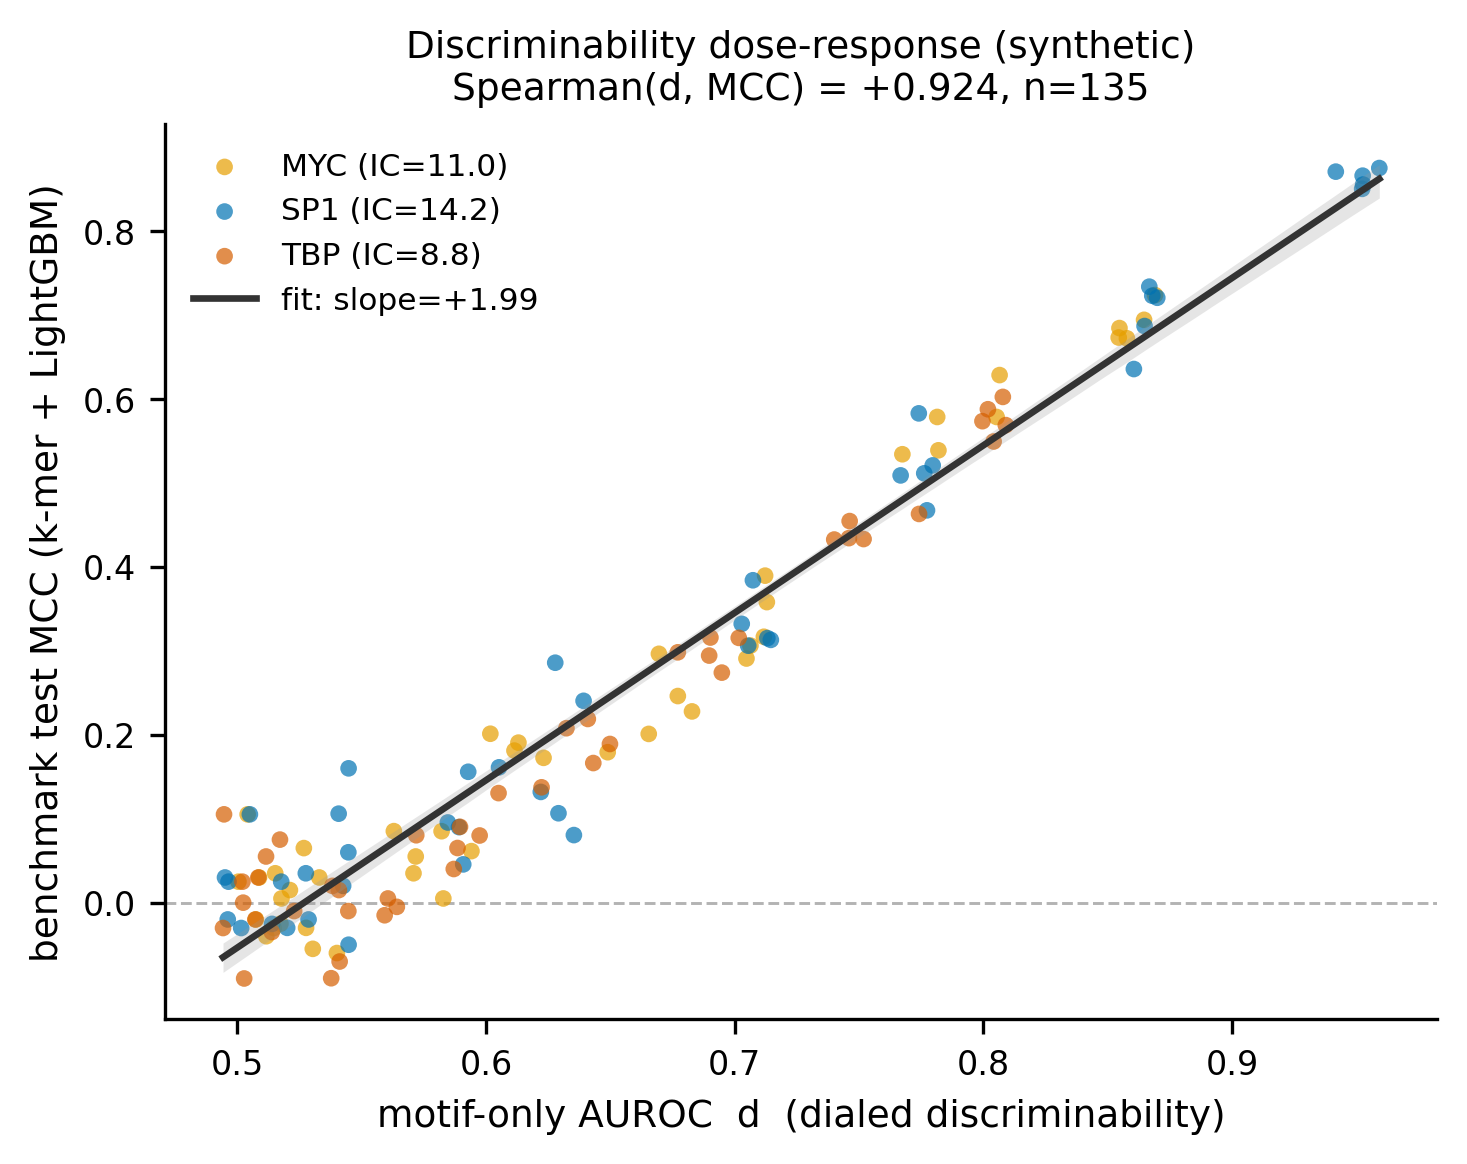
\includegraphics[width=0.52\textwidth]{results/upgrades/figures/disc_dose.png}}
\caption{Route~1 dose-response (semi-synthetic): benchmark MCC vs the dialed motif-only AUROC $d$ for
implanted TF motifs ($n{=}135$: 3 motifs $\times$ 5 seeds $\times$ 9 doses). MCC rises monotonically with
$d$, and the per-motif slopes (SP1/MYC/TBP) overlap, so the law is motif-invariant (Section~\ref{route-1}).
Seed 42.}
\label{fig:dose}
\end{figure}

\subsection{Route 2 --- positional signal, selective and graded}\label{route-2}

Splice sites fail on both suites (\texttt{nt\_splice\_sites\_all} MCC 0.244; motif-only AUROC 0.522, at
chance), consistent with a fixed-position GT--AG consensus the position-blind spectrum discards. Adding a
position-binned spectrum ($B{=}8$) gives a clean \textbf{selective rescue} (paired bootstrap): splice
recovers almost entirely, MCC $0.244\to0.868$ ($\Delta{=}+0.624$, 95\% CI $[0.594, 0.651]$), while every
control barely moves ($|\Delta|\le0.013$, $\sim$50$\times$ smaller). Extended to all 15 tasks the pattern
is \emph{selective} --- one large rescue (splice $\Delta{=}+0.601$, $[0.572, 0.630]$, below the uncapped
$+0.624$ because splice's training set is capped to 20k in this sweep), one marginal gain for the
fixed-position TATA-promoter (\texttt{nt\_promoter\_tata} $\Delta{=}+0.019$, fixed $-25$ to $-30$\,bp
offset), and $|\Delta|\le0.028$ for the other twelve. Within the one responding task the effect is
\emph{graded} in bin resolution: $B\in\{2,4,8,16\}$ grows the splice rescue monotonically
($+0.46, +0.53, +0.60, +0.66$), not one lucky bin. Position is the causal missing ingredient exactly where
fixed-position signal exists, and rescues neither motif-local nor contaminated tasks.

\subsection{Route 3 --- negative-set contamination: existence, mechanism, magnitude,
specificity}\label{route-3}

\textbf{Existence and replication.} The strongest single-motif separator on the failed enhancer datasets
is TATA/TBP, skewed to the \textbf{negative} class. On \texttt{human\_enhancers\_cohn}, negatives carry
far more TATA boxes than positives (TBP hit-count positive mean 0.683 vs negative 1.641; motif-only AUROC
0.371, 95\% CI $[0.365, 0.376]$; TATA-box fraction positive 34.6\% vs negative 57.3\%, an \textbf{excess
of $+22.7\%$}). The same signature appears on the separately-curated \texttt{nt\_enhancers} (TBP positive
0.14 vs negative 0.58; AUROC 0.393 $[0.387, 0.399]$; TATA-box fraction positive 10.6\% vs negative
31.5\%, an excess of $+20.9\%$) --- so the contamination is \textbf{not GB-specific} but a broader
benchmark-design issue. The negatives are systematically more AT-rich (lower GC and CpG O/E;
\texttt{cohn}/\texttt{nt\_enhancers} GC AUROC 0.737/0.822).

\textbf{A benchmark-construction observation (not load-bearing).} Exact full-sequence matching finds 100
of the 400 \texttt{nt\_enhancers} test sequences (25.0\%) are verbatim duplicates of a training sequence,
which would inflate any model's \emph{absolute} \texttt{nt\_enhancers} MCC. It does not affect our
within-split composition analyses (positives vs negatives inside one split), and is restated in the
Limitations.

\textbf{Mechanism: AT-rich background, not TSS leakage.} Recovering GRCh38 coordinates for all
13{,}896 \texttt{cohn} negatives and intersecting with GENCODE v44 TSS \textbf{refutes} a
core-promoter-leakage mechanism: TATA-flagged negatives overlap a TSS ($\pm$500\,bp) in only 1.8\% of
cases, \emph{below} the 3.3\% of non-flagged negatives (0.55$\times$ depletion, Fisher
$p{=}3{\times}10^{-8}$) and far below the 15.6\% positive rate that validates the assay; flagged negatives
near a TSS show no peak at the canonical $-25$ to $-30$\,bp (median $-96$). The excess is thus a
compositional artifact of AT-rich sampling, \emph{not} core-promoter contamination. Extending to
\texttt{nt\_enhancers} by fuzzy minimap2 alignment (mappability 22\%$\to$28.2\%), the flagged class is
likewise TSS-\emph{depleted} (0.6\% vs 1.4\%, $0.46\times$, mirroring \texttt{cohn}), no offset peak ---
\textbf{directionally corroborative but underpowered} (28\% mappable; Fisher $p{=}0.17$).

\textbf{Magnitude: how much of the enhancer signal is composition?} The fully composition-equalized
cleaning matches the negatives' joint GC + 16-dinucleotide distribution to the positives' (SMD
$1.007\to0.059$ for \texttt{cohn}). On the equalized split the TATA and GC motif-only AUROC collapse to
chance (\texttt{cohn} TATA $0.371\to0.500$, GC $0.737\to0.500$; \texttt{nt\_enhancers} TATA
$0.393\to0.494$, GC $0.822\to0.540$) and the $k$-mer MCC collapses onto a composition-only baseline
(\texttt{cohn} $0.461\to0.064$, baseline $0.410\to0.000$). The GC-equalized collapse is \emph{partly true
by construction}, so confirmatory; the assumption-light controls below are the non-circular test. The clean control behaves oppositely: \texttt{drosophila} is
already composition-balanced (the equalizer retains 42.9\% of its negatives vs only 4.5--4.9\% for the
contaminated sets) and retains real signal above composition (MCC $0.398\to0.177$, residual $+0.128$).
The equalized MCC is unpaired and underpowered, so the AUROC collapse is the causal readout. \emph{A second, assumption-light intervention
agrees}: against dinucleotide-shuffled negatives (no mono/dinucleotide composition gap by construction)
the artifact \emph{vanishes} for the contaminated sets (\texttt{cohn} TATA $0.371\to0.551$, GC
$\to0.500$; \texttt{nt\_enhancers} TATA $0.393\to0.507$, GC $\to0.500$), isolating the random-genomic
sampling protocol as the cause; for the control, whose TATA is a genuine positive motif, the TATA AUROC
instead \emph{rises} to 0.749 (Figure~\ref{fig:r3}).

\textbf{Specificity: composition, not the ordered TATA pattern (Figure~\ref{fig:spec}).} A
negative-control-motif panel shows the skew is not manufactured by the scanning procedure and is
composition-driven. Information-content-matched \emph{random} control PWMs produce no class skew
(motif-only AUROC $0.502\pm0.033$ for \texttt{cohn}, $0.507\pm0.016$ for \texttt{nt\_enhancers} --- on
chance), confirming the scan invents no skew. But a \emph{column-scrambled} TBP --- which preserves TBP's
AT-rich per-column composition while destroying the ordered TATA pattern --- stays skewed ($0.376\pm0.017$
and $0.396\pm0.027$, essentially equal to real TATA). The negative-set skew is therefore driven by AT-rich
\emph{composition}, not the ordered TATA pattern, corroborating the coordinate analysis. A built-in positive control behaves correctly: real TATA on
\texttt{nt\_promoter\_tata} skews to the \emph{positives} (AUROC 0.589, $[0.577, 0.600]$). The collapse is
threshold-robust: sweeping the TATA threshold across 0.8--1.5\,bits/pos, the equalized TATA AUROC stays on
chance throughout (\texttt{cohn} $[0.485, 0.503]$, \texttt{nt\_enhancers} $[0.490, 0.501]$) while the
original is neg-skewed at every threshold --- the headline does not depend on the 1.3\,bits/pos point.

\textbf{The interventional headline.} Removing the excess TATA-bearing negatives
(TATA-flag cleaning) drops 22.2\% of \texttt{cohn} and 20.8\% of \texttt{nt\_enhancers} negatives and moves
the TATA motif-only AUROC toward 0.5 (\texttt{cohn} $0.371\to0.435$; \texttt{nt\_enhancers}
$0.393\to0.485$; seed-invariant; GC-matched cleaning agrees, $\to$0.423/0.458). The apparent benchmark MCC
also drops (\texttt{cohn} $0.461\to0.407$; \texttt{nt\_enhancers} $0.514\to0.459$), consistent with partial
inflation, though the MCC is unpaired so the AUROC collapse (and the paired FM \texttt{test\_effect} below)
is the causal readout. The
\emph{TATA-clean} control \texttt{drosophila\_enhancers\_stark} (a hard task with no negative-set TATA
excess) behaves as required: the identical procedure removes 0.0\% of its negatives and
leaves its TATA AUROC (0.539) and MCC unchanged. We grade the verdict: \texttt{cohn} and
\texttt{nt\_enhancers} are robust; \texttt{human\_enhancers\_ensembl} is weaker/suggestive (excess
$+10.8\%$). Both robust benchmarks draw random AT-rich genomic negatives; the shuffled-negative result shows the
artifact is a property of that sampling practice, not of either dataset.

\begin{figure}[t]
\centerline{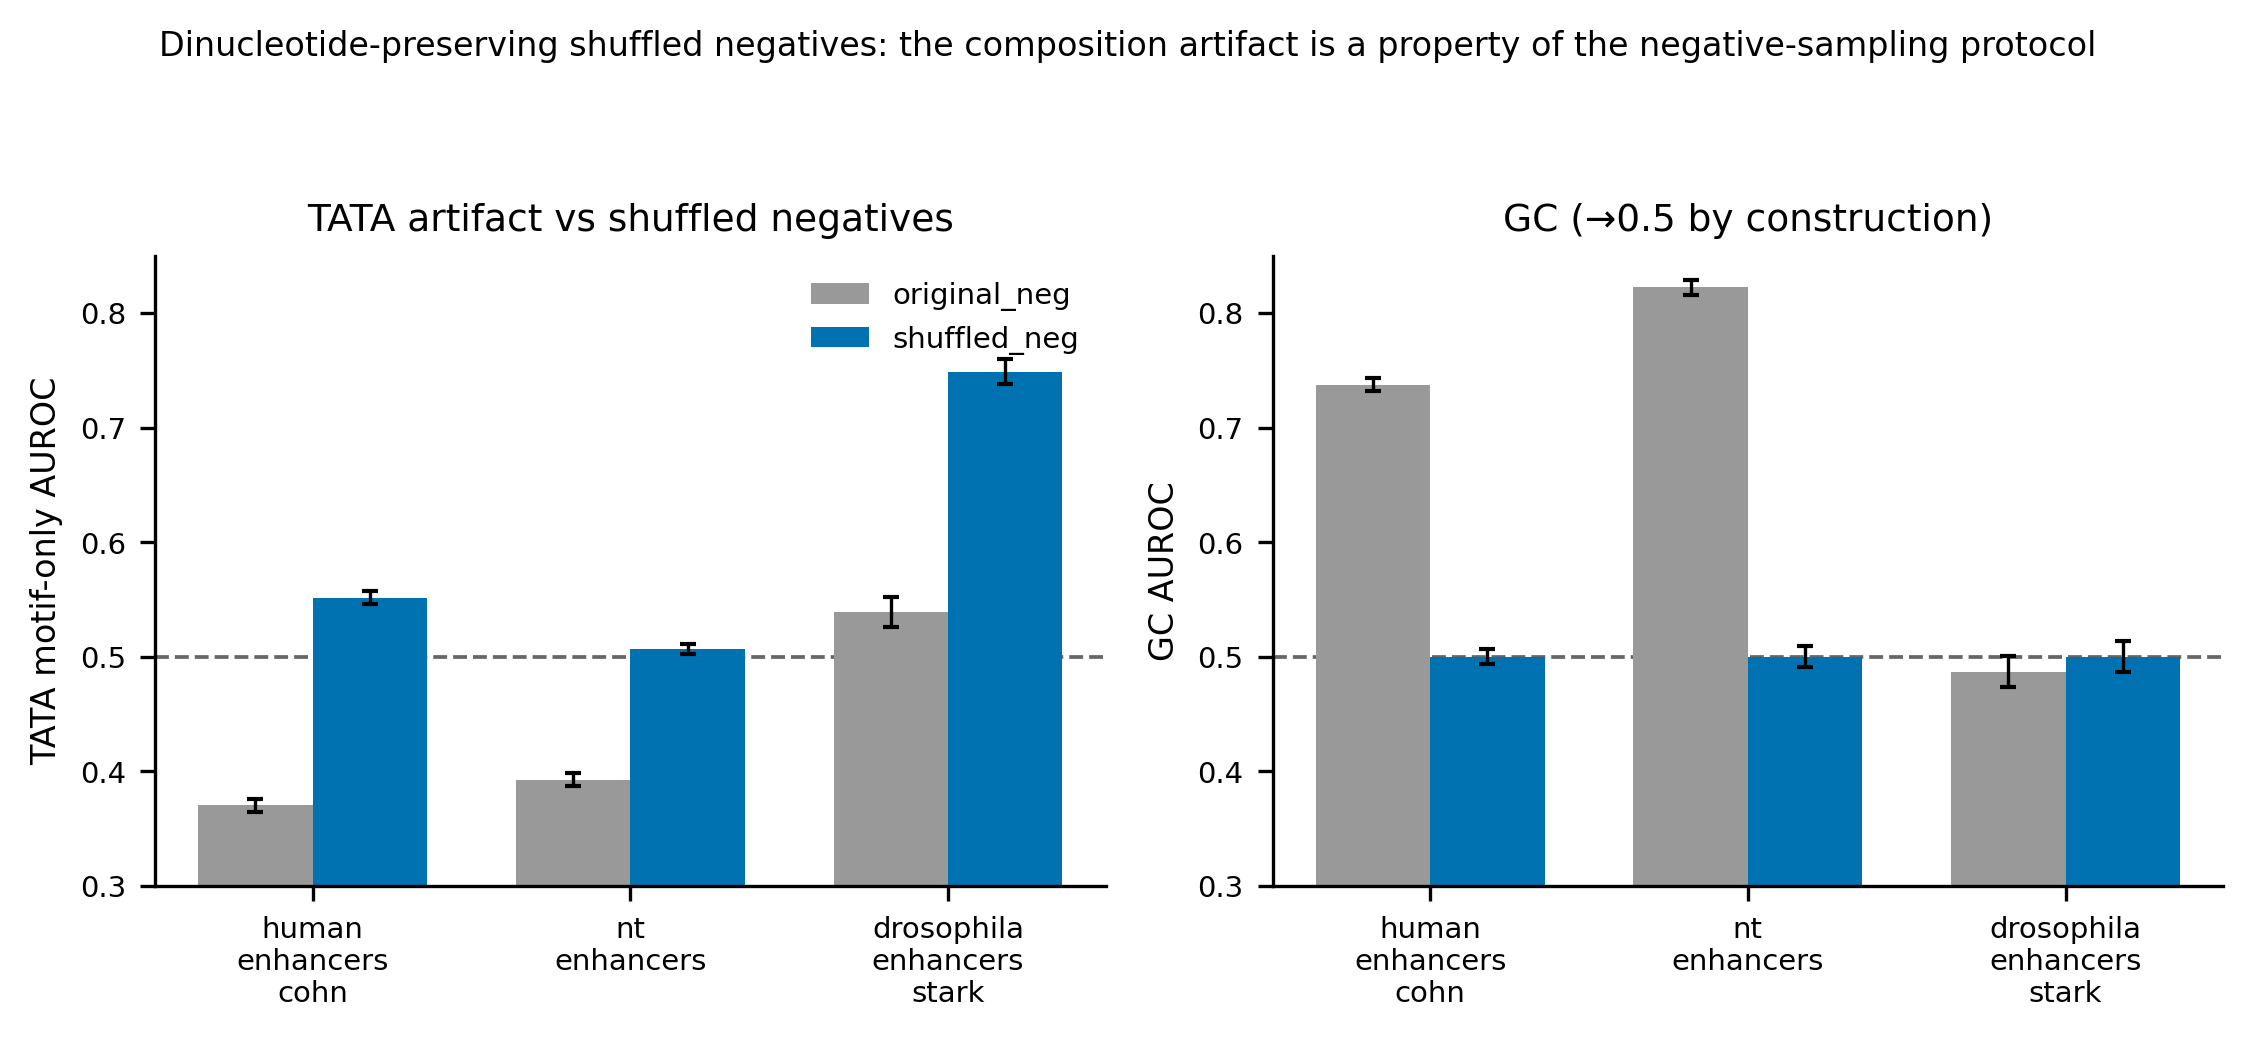
\includegraphics[width=0.52\textwidth]{results/upgrades/figures/shuffled_neg.png}}
\caption{Route~3 magnitude via dinucleotide-shuffled negatives. TATA (left) and GC (right) motif-only
AUROC against real negatives vs dinucleotide-preserving shuffles of the positives. For the contaminated
sets the artifact \emph{vanishes} to chance once the composition gap is removed; for the clean control
(\texttt{drosophila}), whose TATA is a genuine positive-class motif, it instead rises. Seed 42, 1000-bootstrap.}
\label{fig:r3}
\end{figure}

\begin{figure}[t]
\centerline{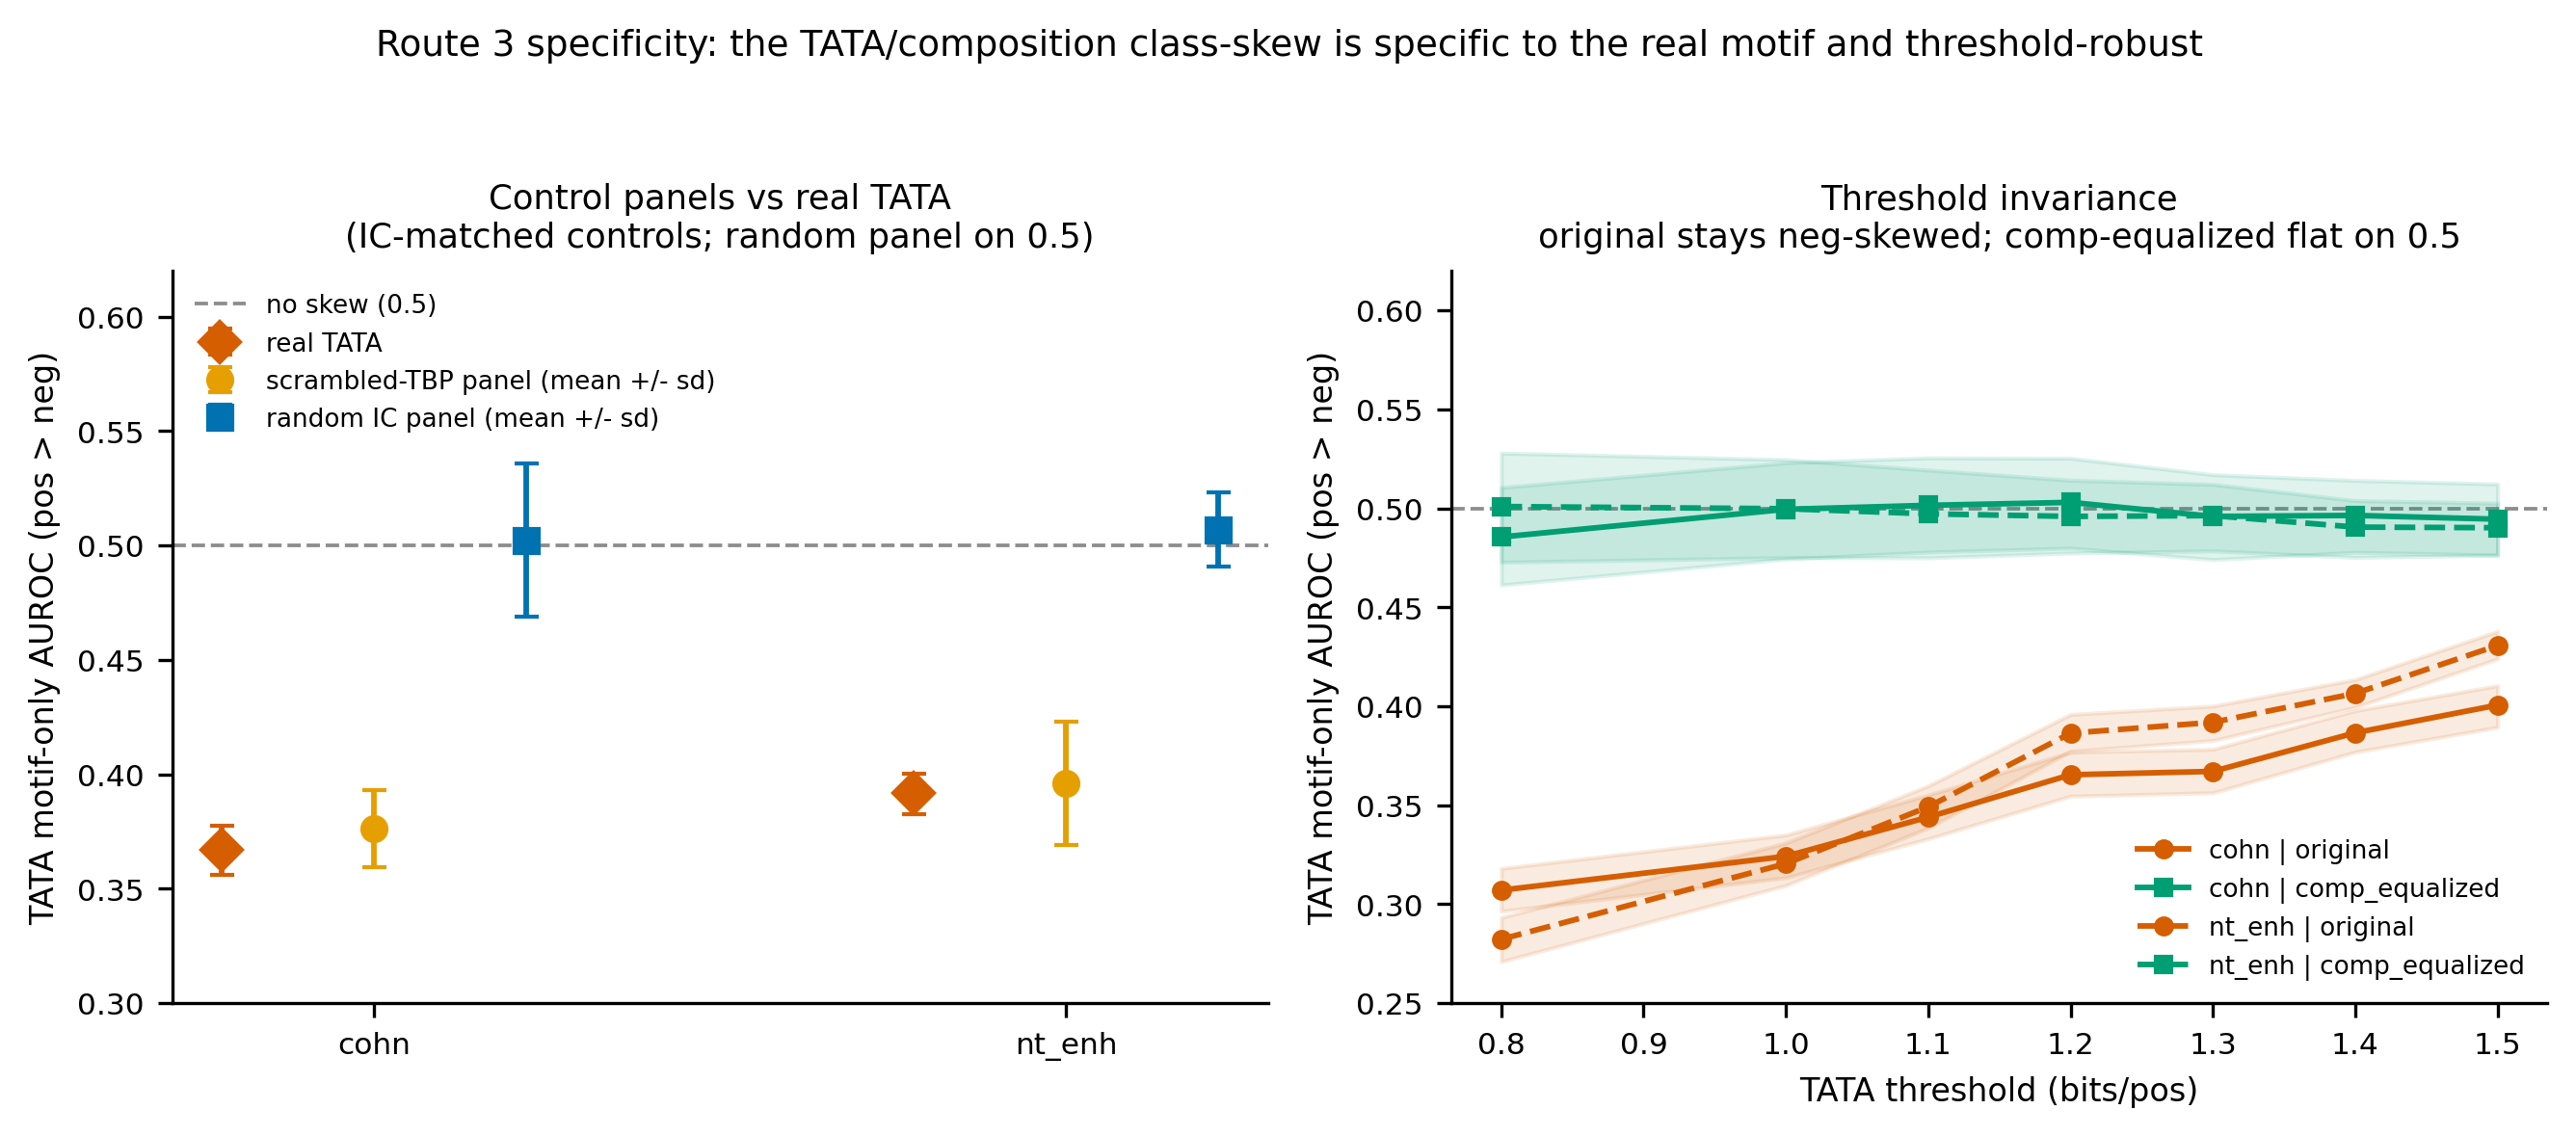
\includegraphics[width=0.63\textwidth]{results/upgrades/figures/route3_specificity.png}}
\caption{Route~3 specificity. \textbf{(Left)} Random-IC control PWMs land on chance --- the scan
manufactures no skew --- while column-scrambled-TBP PWMs (composition preserved, order destroyed) stay
skewed $\approx$ real TATA: composition-driven, not order-driven. \textbf{(Right)} Across 0.8--1.5\,bits/pos
the composition-equalized TATA AUROC stays on chance, the original neg-skewed. Seed 42.}
\label{fig:spec}
\end{figure}

\subsection{Cross-architecture frozen-FM probe: an existence proof}\label{fm-probe}

The Route-3 results above are computed from the sequences themselves and so apply to any model, but they
do not by themselves show that a \emph{pretrained} model exploits the composition shortcut. We provide
that as an existence proof with frozen-FM probes, and we are explicit that it is a \textbf{conservative
lower bound}, not a measurement of the artifact's magnitude (which lives in Route~3).

\textbf{Paired evaluation.} We train a head on a frozen FM's embeddings and measure how much enhancer
AUROC the \emph{same fixed head} loses when composition-biased negatives are removed from the \emph{test}
set (\texttt{test\_effect}), on a retained GC-matched subset so the test set is held fixed (nested paired
bootstrap, 1000 resamples); a flat control gives \texttt{test\_effect} $\approx 0$.

\textbf{HyenaDNA.} On HyenaDNA-tiny embeddings the fixed head loses significant enhancer AUROC when
composition is removed: \texttt{test\_effect} $= -0.048$ (95\% CI $[-0.053, -0.043]$) on \texttt{cohn}
and $-0.079$ ($[-0.107, -0.056]$) on \texttt{nt\_enhancers} (both CIs exclude 0), while the clean control
\texttt{drosophila} is flat, $+0.005$ ($[-0.003, +0.014]$, CI includes 0). The effect is
\textbf{head-invariant} --- an LR head gives the same signs and significance --- so it lives in the frozen
representation, not the read-out head.

\textbf{DNABERT-2 (second architecture), with its own flat control.} We repeat the identical paired
evaluation with an architecturally-unrelated FM, DNABERT-2-117M (a bidirectional BPE BERT), on the two
short datasets. DNABERT-2 loses near-identical AUROC: \texttt{test\_effect} $= -0.047$
($[-0.051, -0.042]$, mean-pool) and $-0.046$ ($[-0.052, -0.042]$, [CLS]) on \texttt{cohn}, and $-0.072$
($[-0.100, -0.049]$) and $-0.077$ ($[-0.106, -0.051]$) on \texttt{nt\_enhancers}; all CIs exclude 0, both
poolings, both heads (Figure~\ref{fig:cross}). DNABERT-2 cannot use the long \texttt{drosophila} control
(its sequences exceed the 512-token context), so we give it \emph{its own} flat control by a
composition-representative placebo: on the same frozen \texttt{cohn} head we remove the \emph{same number}
of test negatives that the GC-matched cleaning removes (1148), but chosen at random (representative)
rather than the AT-rich tail. This placebo is flat across all four head/pooling combinations
(every \texttt{test\_effect} CI includes 0), whereas removing the composition-biased negatives costs
$-0.047$ --- so DNABERT-2's loss is specific to \emph{composition} removal, not to shrinking the negative
set.\footnote{The naive flat control --- a dinucleotide-shuffled-negative version of \texttt{cohn} ---
is degenerate here: each shuffled negative has the same per-sequence GC as its positive, so GC-matched
cleaning removes nothing and \texttt{test\_effect} is trivially 0. The representative-removal placebo is
the non-degenerate control.}

\textbf{Interpretation.} Two architecturally-unrelated pretrained FMs lose nearly the same significant
enhancer AUROC when the composition artifact is removed. That a pretrained model demonstrably rides the
shortcut is the claim; the small AUROC delta is a \emph{floor}, not the artifact's size (which is large;
Section~\ref{route-3}).

\begin{figure}[t]
\centerline{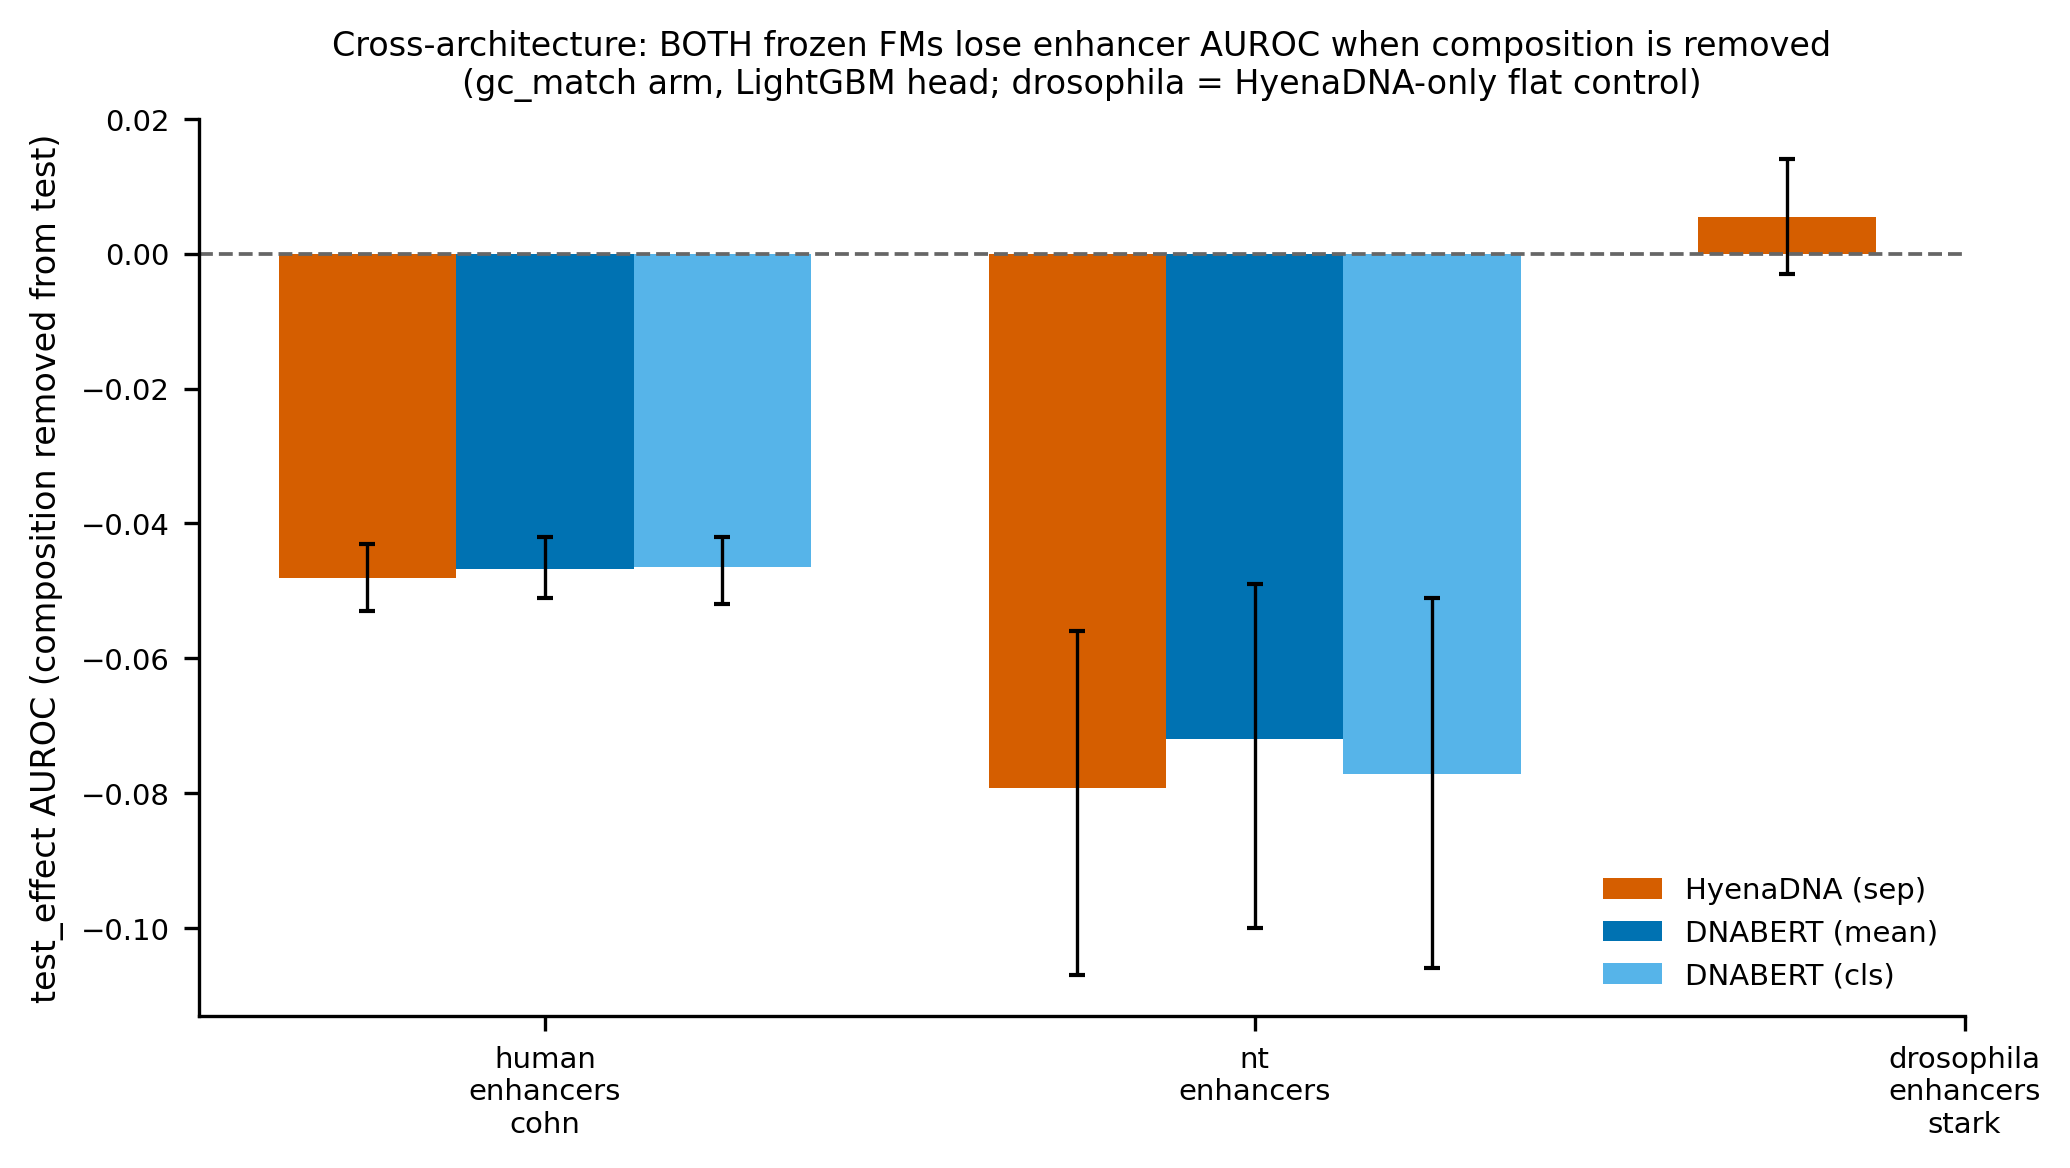
\includegraphics[width=0.50\textwidth]{results/upgrades/figures/fm_cross_architecture.png}}
\caption{Cross-architecture frozen-FM existence proof: the fixed FM head's enhancer AUROC loss
(\texttt{test\_effect}, GC-matched arm) when composition is removed, for HyenaDNA and DNABERT-2 (LightGBM
head, 95\% bootstrap CIs). Both lose near-identical significant AUROC on the contaminated sets
(\texttt{cohn}, \texttt{nt\_enhancers}); the HyenaDNA control (\texttt{drosophila}) and the DNABERT-2
placebo are flat. Seed 42.}
\label{fig:cross}
\end{figure}

\subsection{Robustness}\label{robustness}

The route assignments are stable under the choices a skeptic would question. A 5-seed LightGBM loop leaves
the benchmark MCC seed-invariant (max SD 0.013 across eight key tasks), with the solved/hard tier stable
for 7/8 (the lone flip, \texttt{nt\_enhancers}, sits on the 0.5 cutoff). Across model families the per-task
solved/hard tier agrees on 13/15 tasks for LR vs LightGBM and 3/3 for LightGBM vs the frozen FM-probe head;
disagreements are capacity-driven or 0.5-boundary, not route changes, and the FM-probe independently agrees
the enhancer tasks are hard --- cross-family evidence without a from-scratch CNN. The FM composition-removal effect is head-invariant (Section~\ref{fm-probe}) and the
Route-1 slope is motif-invariant (Section~\ref{route-1}).

\section{Discussion}\label{discussion}

\textbf{For benchmark design.} The taxonomy gives a model-independent vocabulary for \emph{why} a genomic
task is easy or hard: a high score can reflect a clean class-specific motif (the promoter / GC-box case);
a low score, diffuse or combinatorial signal, a fixed-position motif a representation discards, or ---
most consequentially --- a negative set whose composition itself produces the discriminative signal.

\textbf{The contamination implication: benchmark design, not dataset corruption.} Two enhancer benchmarks
reward separating enhancers from negatives partly on an excess TATA/AT-rich signal the coordinate analysis
shows is background, not core-promoter leakage --- available to any model, and ridden by our classifier and
two frozen FMs alike. But enhancer positives \emph{are} GC-rich relative to genomic background as a real
biological property, so the composition gap is a genuine feature of the two classes, \textbf{not a
corruption introduced in dataset construction}: the critique is one of \emph{benchmark design} --- the task
is partly solvable by a trivial composition axis that does not test regulatory grammar. The interventions
drive the artifact to chance while residual enhancer signal survives in the control, so the shortcut is
separable from genuine signal. We fixed the flagging criterion, overlap test, and thresholds before
obtaining the coordinates; the result refuted our initial core-promoter prior.

\textbf{Limitations (reported straight).} (i)~Route~1 rests on the causal dose-response, with the
real-task correlation and held-out test (Section~\ref{route-1}) as corroboration only --- the latter's
$R^2$ CI includes 0 at $n{=}11$, so we lead with the stable MAE. (ii)~The FM
result is a frozen-feature existence proof (no fine-tuning, no leaderboard scores), so its effect on any
specific fine-tuned FM score is unmeasured. (iii)~The
composition-equalized MCC is unpaired and underpowered, so the AUROC collapse is the causal readout; as the
GC-driven collapse is partly true by construction, the dinucleotide-shuffle and column-scrambled-TBP
controls are the primary non-circular specificity evidence (Section~\ref{route-3}). (iv)~We read each benchmark at its \emph{provided} split without homology
re-clustering: an $8$-mer-Jaccard audit finds the flagship \texttt{cohn} redundancy-clean (0.11\%
$\ge$0.7 near-duplicate) but \texttt{human\_nontata\_promoters} (41\% $\ge$0.7) and \texttt{nt\_enhancers}
(25\% verbatim) inflated, so their \emph{absolute} Table~\ref{tab:land} MCCs are partly homology-inflated
--- shifting those numbers but not the route assignments, within-split interventions, or contamination
magnitude, and the correlation strengthens when they are dropped (Section~\ref{route-1}).

\textbf{Artifact and reproducibility.} We release cleaned train/test splits (\texttt{sequence,label}) for
\texttt{human\_enhancers\_cohn}, \texttt{nt\_enhancers}, and the \texttt{drosophila\_enhancers\_stark}
control (TATA-flag, GC-matched, and composition-equalized variants), the frozen-FM embedding cache with
manifest (regenerating the entire FM result with zero PyTorch; Section~\ref{fm-probe-method}), and the
\texttt{diagnose.py} CLI as a route-labeled report card for contamination-free enhancer evaluation
(\url{https://github.com/rikhinkavuru/gb_kmer_benchmark}).

\textbf{Future work.} Fine-tuning foundation models on the original versus cleaned splits to measure the
artifact's effect on FM scores directly; and extending the taxonomy with additional representations.

\section{Conclusion}\label{conclusion}

Treating a simple, interpretable, CPU-only classifier as a diagnostic lens, we give a three-route
taxonomy --- shared-motif, positional, contamination --- for why genomic sequence-classification tasks
fail, each confirmed causally: Route~1 by a semi-synthetic dose-response (Section~\ref{route-1}) that
corroborates out-of-sample and strengthens on the homology-clean subset; Route~2 by a selective, bin-graded positional
rescue; and Route~3 by composition-equalized cleaning, dinucleotide-shuffled negatives, and a
negative-control-motif panel showing two enhancer benchmarks carry an AT-rich \emph{benchmark-design}
confound in their negatives --- not core-promoter leakage, and not dataset corruption --- of large
magnitude. As an existence proof, two architecturally-unrelated frozen FMs lose near-identical,
significant enhancer AUROC when the artifact is removed, each against its own flat control. We release
cleaned splits, the frozen-FM embedding cache, and a
diagnostic tool for contamination-free evaluation.

\begin{thebibliography}{99}
\bibitem{gb} K. Gre\v{s}ov\'{a}, V. Martinek, D. \v{C}ech\'{a}k, P. \v{S}ime\v{c}ek, and P. Alexiou,
Genomic Benchmarks: a collection of datasets for genomic sequence classification, {\it BMC Genomic Data}
{\bf 24}, 25 (2023).
\bibitem{nt} H. Dalla-Torre {\it et al.}, The Nucleotide Transformer: building and evaluating robust
foundation models for human genomics, {\it Nature Methods} (2024).
\bibitem{dnabert} Y. Ji, Z. Zhou, H. Liu, and R.~V. Davuluri, DNABERT: pre-trained Bidirectional Encoder
Representations from Transformers model for DNA-language in genome, {\it Bioinformatics} {\bf 37}(15),
2112 (2021).
\bibitem{dnabert2} Z. Zhou, Y. Ji, W. Li, P. Dutta, R. Davuluri, and H. Liu, DNABERT-2: Efficient
Foundation Model and Benchmark for Multi-Species Genome, in {\it Int. Conf. on Learning Representations
(ICLR)} (2024), arXiv:2306.15006.
\bibitem{hyenadna} E. Nguyen {\it et al.}, HyenaDNA: Long-Range Genomic Sequence Modeling at Single
Nucleotide Resolution, in {\it Advances in Neural Information Processing Systems (NeurIPS)} (2023).
\bibitem{caduceus} Y. Schiff {\it et al.}, Caduceus: Bi-Directional Equivariant Long-Range DNA Sequence
Modeling, in {\it Int. Conf. on Machine Learning (ICML)} (2024).
\bibitem{lightgbm} G. Ke {\it et al.}, LightGBM: A Highly Efficient Gradient Boosting Decision Tree, in
{\it Advances in Neural Information Processing Systems (NeurIPS)} (2017).
\bibitem{sklearn} F. Pedregosa {\it et al.}, Scikit-learn: Machine Learning in Python, {\it J. Machine
Learning Research} {\bf 12}, 2825 (2011).
\bibitem{jaspar} I. Rauluseviciute {\it et al.}, JASPAR 2024: 20th anniversary of the open-access database
of transcription factor binding profiles, {\it Nucleic Acids Research} {\bf 52}(D1), D174 (2024).
\bibitem{mcc} D. Chicco and G. Jurman, The advantages of the Matthews correlation coefficient (MCC) over
F1 score and accuracy in binary classification evaluation, {\it BMC Genomics} {\bf 21}, 6 (2020).
\bibitem{bh} Y. Benjamini and Y. Hochberg, Controlling the false discovery rate: a practical and powerful
approach to multiple testing, {\it J. Royal Statistical Society: Series B} {\bf 57}(1), 289 (1995).
\bibitem{pyjaspar} A. Khan, pyJASPAR: a Pythonic interface to JASPAR transcription factor motifs, Zenodo
(2021), doi:10.5281/zenodo.4509415.
\bibitem{convnova} Y. Bo {\it et al.}, Revisiting Convolution Architecture in the Realm of DNA Foundation
Models, in {\it Int. Conf. on Learning Representations (ICLR)} (2025), arXiv:2502.18538.
\bibitem{embed} N. Datta, S. Shatabda, and M.~S. Rahman, Embedding Is (Almost) All You Need:
Retrieval-Augmented Inference for Generalizable Genomic Prediction Tasks, arXiv:2508.04757 (2025).
\bibitem{caofullwood} F. Cao and M.~J. Fullwood, Inflated performance measures in enhancer-promoter
interaction-prediction methods, {\it Nature Genetics} {\bf 51}(8), 1196 (2019).
\bibitem{rosenbaum} P.~R. Rosenbaum and D.~B. Rubin, The central role of the propensity score in
observational studies for causal effects, {\it Biometrika} {\bf 70}(1), 41 (1983).
\bibitem{altschul} S.~F. Altschul and B.~W. Erikson, Significance of nucleotide sequence alignments: a
method for random sequence permutation that preserves dinucleotide and codon usage, {\it Molecular
Biology and Evolution} {\bf 2}(6), 526 (1985).
\bibitem{minimap2} H. Li, Minimap2: pairwise alignment for nucleotide sequences, {\it Bioinformatics}
{\bf 34}(18), 3094 (2018).
\bibitem{lee2011} D. Lee, R. Karchin, and M.~A. Beer, Discriminative prediction of mammalian enhancers
from DNA sequence, {\it Genome Research} {\bf 21}(12), 2167 (2011).
\bibitem{ghandi2014} M. Ghandi, D. Lee, M. Mohammad-Noori, and M.~A. Beer, Enhanced Regulatory Sequence
Prediction Using Gapped $k$-mer Features, {\it PLoS Computational Biology} {\bf 10}(7), e1003711 (2014).
\bibitem{ghandi2016} M. Ghandi {\it et al.}, gkmSVM: an R package for gapped-kmer SVM, {\it
Bioinformatics} {\bf 32}(14), 2205 (2016).
\bibitem{deepromoter} M. Oubounyt, Z. Louadi, H. Tayara, and K.~T. Chong, DeePromoter: Robust Promoter
Predictor Using Deep Learning, {\it Frontiers in Genetics} {\bf 10}, 286 (2019),
doi:10.3389/fgene.2019.00286.
\bibitem{krutzfeldt2020} L.-M. Kr\"utzfeldt, M. Schubach, and M. Kircher, The impact of different negative
training data on regulatory sequence predictions, {\it PLoS ONE} {\bf 15}(12), e0237412 (2020),
doi:10.1371/journal.pone.0237412.
\bibitem{feng2025} J. Feng {\it et al.}, Benchmarking DNA foundation models for genomic and genetic tasks,
{\it Nature Communications} {\bf 16}(1), 10780 (2025), doi:10.1038/s41467-025-65823-8.
\end{thebibliography}

\end{document}
